\documentclass{standalone}
%
\usepackage{tikz}
\usetikzlibrary{backgrounds}
%
\usepackage{xcolor}
\definecolor{space}{HTML}{0A2543}
\definecolor{earth}{HTML}{0089FA}
\definecolor{mars}{HTML}{DC7B4E}
%
\title{Mars}
\begin{document}
	\tikzset{partial ellipse/.style args = {#1:#2:#3}{insert path={+ (#1:#3) arc (#1:#2:#3)}}}
	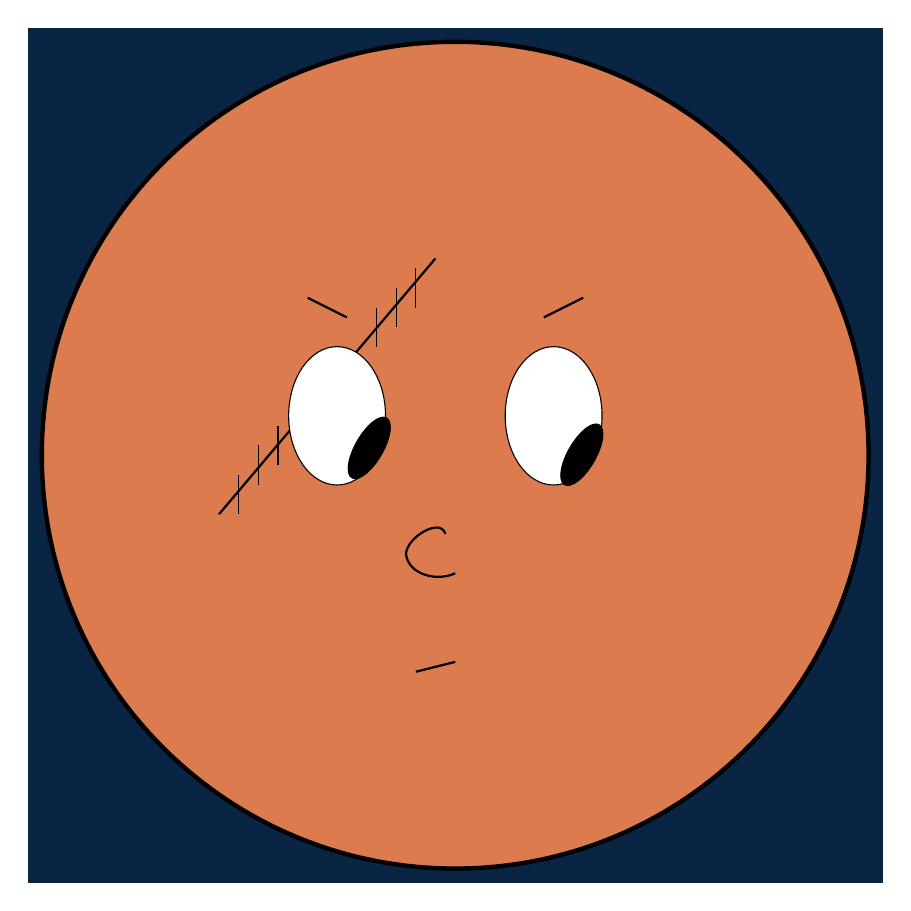
\begin{tikzpicture}[background rectangle/.style={fill=space},show background rectangle,]
		\begin{scope}[scale=2.5]
			\coordinate (E) at (2.6,0.4);
			\coordinate (F) at (3.7,0.7);
			\draw[fill=mars,ultra thick] (3,0.5) circle (2.1cm);
			%scar
			\draw[-,thick] (1.8,0.2) -- (2.9,1.5);
			\draw[-] (1.9,0.2) -- (1.9,0.4);
			\draw[-] (2,0.35) -- (2,0.55);
			\draw[-] (2.1,0.45) -- (2.1,0.65);
			\draw[-] (2.6,1.05) -- (2.6,1.25);
			\draw[-] (2.7,1.15) -- (2.7,1.35);
			\draw[-] (2.8,1.25) -- (2.8,1.45);
			%eyebrows
			\draw[-,thick] (2.25,1.3) -- (2.45,1.2);
			\draw[-,thick] (3.45,1.2) -- (3.65,1.3);
			%nose
			\draw[-,thick] (2.95,0.1) to[out=105,in=85] (2.75,0) to[out=275,in=205] (3,-0.1);
			%mouth
			\draw[-,thick] (2.8,-0.6) -- (3,-0.55);
			%eyes
			\draw[fill=white] (2.4,0.7) ellipse (7pt and 10pt);
			\draw[fill=white] (3.5,0.7) ellipse (7pt and 10pt);
			\draw[fill=black,rotate around={-30:(E)}] (2.5,0.5) ellipse (2pt and 5pt);
			\draw[fill=black,rotate around={-30:(F)}] (3.75,0.5) ellipse (2pt and 5pt);
		\end{scope}
	\end{tikzpicture}
\end{document}